% layers
\pgfdeclarelayer{background}
\pgfdeclarelayer{foreground}
\pgfsetlayers{background, main, foreground}

% styles
\tikzstyle{box} = [draw, text centered, rounded corners]
\tikzstyle{register} = [box, fill=white, minimum height=2em, minimum width=4em]
\tikzstyle{processor} = [draw, fill=blue!10, rounded corners]
\tikzstyle{buffer} = [processor, fill=red!10, dashed]

% distances
\def\blockdist{3}
\def\borderdist{0.2}

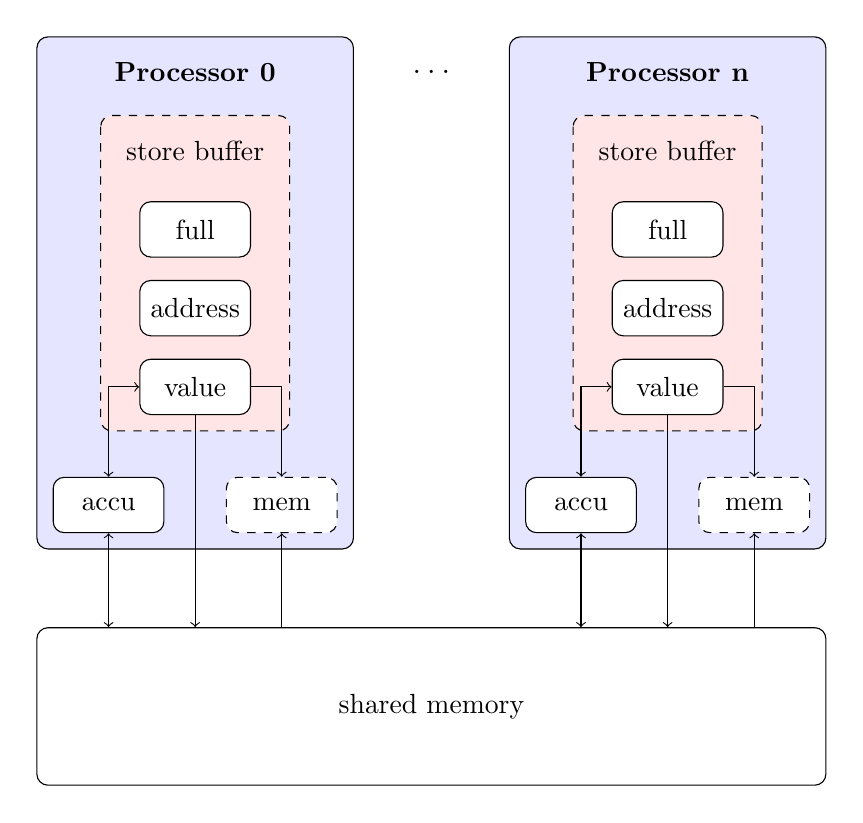
\begin{tikzpicture}

  % processor 0 %%%%%%%%%%%%%%%%%%%%%%%%%%%%%%%%%%%%%%%%%%%%%%%%%%%%%%%%%%%%%%%%
  \path (0, 0) node (title-0) [] {\textbf{Processor 0}};

  % store buffer
  \path (title-0)+(0, -1) node (sb-0) [] {store buffer};
  \path (sb-0)+(0, -1) node (full-0) [register] {full};
  \path (full-0)+(0, -1) node (adr-0) [register] {address};
  \path (adr-0)+(0, -1) node (val-0) [register] {value};

  % registers
  \path (val-0)+(-1.1, -1.5) node (accu-0) [register] {accu};
  \path (val-0)+(1.1, -1.5) node (mem-0) [register, dashed] {mem};

  % paths
  \path [draw, <->] (val-0.west) -- (val-0.west -| accu-0.north) -- (accu-0.north);
  \path [draw, ->] (val-0.east) -- (val-0.east -| mem-0.north) -- (mem-0.north);

  \begin{pgfonlayer}{background}
    % bounding box
    \path (accu-0.west |- title-0.north)+(-\borderdist, \borderdist) node (a) {};
    \path (mem-0.south east)+(\borderdist, -\borderdist) node (b) {};
    \path [processor] (a) rectangle (b);

    % top left heap coordinate
    \path (a |- b)+(0, -1) node (tlh) {};

    % store buffer box
    \path (sb-0.north west)+(-\borderdist, \borderdist) node (a) {};
    \path (val-0.south -| sb-0.east)+(\borderdist, -\borderdist) node (b) {};
    \path [buffer] (a) rectangle (b);
  \end{pgfonlayer}

  % dots %%%%%%%%%%%%%%%%%%%%%%%%%%%%%%%%%%%%%%%%%%%%%%%%%%%%%%%%%%%%%%%%%%%%%%%
  \path (title-0)+(\blockdist, 0) node (dots) [] {\large $\ldots$};

  % processor n %%%%%%%%%%%%%%%%%%%%%%%%%%%%%%%%%%%%%%%%%%%%%%%%%%%%%%%%%%%%%%%%
  \path (dots)+(\blockdist, 0) node (title-n) [] {\textbf{Processor n}};

  % store buffer
  \path (title-n)+(0, -1) node (sb-n) [] {store buffer};
  \path (sb-n)+(0, -1) node (full-n) [register] {full};
  \path (full-n)+(0, -1) node (adr-n) [register] {address};
  \path (adr-n)+(0, -1) node (val-n) [register] {value};

  % registers
  \path (val-n)+(-1.1, -1.5) node (accu-n) [register] {accu};
  \path (val-n)+(1.1, -1.5) node (mem-n) [register, dashed] {mem};

  % paths
  \path [draw, <->] (val-n.west) -- (val-n.west -| accu-n.north) -- (accu-n.north);
  \path [draw, ->] (val-n.east) -- (val-n.east -| mem-n.north) -- (mem-n.north);

  \begin{pgfonlayer}{background}
    % bounding box
    \path (accu-n.west |- title-n.north)+(-\borderdist, \borderdist) node (a) {};
    \path (mem-n.south east)+(\borderdist, -\borderdist) node (b) {};
    \path [processor] (a) rectangle (b);

    % bottom right heap coordinate
    \path (b)+(0, -\blockdist) node (brh) {};

    % store buffer box
    \path (sb-n.north west)+(-\borderdist, \borderdist) node (a) {};
    \path (val-n.south -| sb-n.east)+(\borderdist, -\borderdist) node (b) {};
    \path [buffer] (a) rectangle (b);
  \end{pgfonlayer}

  % heap %%%%%%%%%%%%%%%%%%%%%%%%%%%%%%%%%%%%%%%%%%%%%%%%%%%%%%%%%%%%%%%%%%%%%%%
  \path [box] (tlh) rectangle node (heap) [minimum height=2cm] {shared memory} (brh);

  % paths
  \path [draw, ->] (val-0) -- (heap.north -| val-0);
  \path [draw, <->] (accu-0) -- (heap.north -| accu-0);
  \path [draw, <-] (mem-0) -- (heap.north -| mem-0);

  \path [draw, ->] (val-n) -- (heap.north -| val-n);
  \path [draw, <->] (accu-n) -- (heap.north -| accu-n);
  \path [draw, <-] (mem-n) -- (heap.north -| mem-n);

\end{tikzpicture}
